% =====================================================================
%  Material suplementario -- version en ingles de CSMIO2026_suplemento.tex
%  Espejo: mismas secciones, mismas etiquetas (\label), mismos cuadros y
%  figuras, misma numeracion S1..S9 / Figura S1..S5. Los comentarios
%  siguen en espanol porque son notas de trabajo.
%
%  Compila por separado (main_suplemento_en.tex). Las referencias cruzadas
%  al articulo principal se escriben a mano porque son dos documentos.
%
%  Diferencias con la version en espanol, todas de idioma:
%     - sin babel-spanish: no hace falta \decimalpoint ni cuidar que
%       \,\% quede fuera de modo matematico. Porcentajes como 15.0\%.
%     - Separador de miles: SIEMPRE coma (3,003 series; 4,708 series).
%     - "Cuadro"/"Figura"/"Seccion" pasan a Table/Figure/Section solo
%       donde estan escritos a mano; el \caption lo resuelve la clase.
% =====================================================================
\title{Supplementary material\\
       \large How far the structure of a series supports model choice,
       and why it stops there}
\author{Jorge Andres Pe\~na Araya \and Esther Segura P\'erez}
\date{Universidad Nacional Aut\'onoma de M\'exico (UNAM)}
\maketitle

\renewcommand{\thetable}{S\arabic{table}}
\renewcommand{\thefigure}{S\arabic{figure}}
\renewcommand{\thesection}{S\arabic{section}}
\setcounter{section}{0}

\noindent
This document gathers the supporting material of the article: the composition of the
feature vector, the validation of the benchmark, the breakdown by model and frequency,
the configuration under which each model was run, and the details of the computing
environment. None of what follows is needed to follow the argument; all of it is needed
to reproduce it.

\section{Composition of the feature vector, and validations}

The items in this section are cited from the main article.

\begin{table}[htbp]
\centering
\caption{Families of structural features.}
\label{tab:familias}
\begin{tabular}{p{0.30\linewidth}p{0.62\linewidth}}
\toprule
\textbf{Family} & \textbf{Descriptors} \\
\midrule
Distribution shape   & Skewness, kurtosis, Shannon entropy, spectral entropy \\
Local irregularity   & Share of outliers, turning points, changepoints \\
Complexity           & Hurst exponent, robust entropy \\
Temporal dependence  & ACF and PACF at several lags, autocorrelation decay \\
Trend                & Slope, linear $R^{2}$, quadratic gain \\
Seasonality (STL)    & Trend strength, seasonal strength \\
Dominant frequency   & Energy ratio of the dominant spectral peak \\
Stationarity         & ADF, KPSS, indicator of conflict between the two \\
First differences    & Variance ratio, skewness, entropy \\
\bottomrule
\end{tabular}
\end{table}

\begin{table}[htbp]
\centering
\caption{Validation of the Naive2 benchmark against the published values.}
\label{tab:naive2}
\begin{tabular}{lrrr}
\toprule
\textbf{Frequency} & \textbf{Replicated sMAPE} & \textbf{Published sMAPE} & \textbf{Difference} \\
\midrule
Yearly      & 16.342 & 16.342 & $0.000$ \\
Quarterly   & 11.024 & 11.012 & $+0.012$ \\
Monthly     & 14.385 & 14.427 & $-0.042$ \\
Weekly      &  9.161 &  9.161 & $0.000$ \\
Daily       &  3.045 &  3.045 & $0.000$ \\
Hourly      & 18.616 & 18.383 & $+0.233$ \\
\midrule
\textbf{Overall} & \textbf{13.548} & \textbf{13.564} & $\mathbf{-0.016}$ \\
\bottomrule
\end{tabular}
\end{table}



\begin{figure}[htbp]
\centering
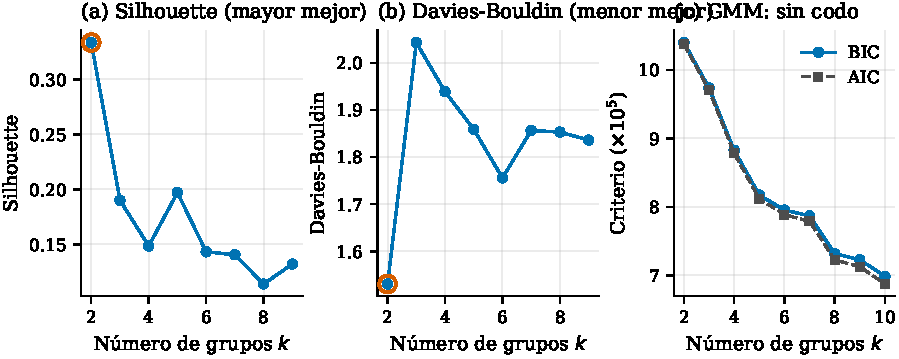
\includegraphics[width=\linewidth]{figuras/fig2_seleccion_k.pdf}
\caption{Choosing the number of groups. (a) Silhouette and (b) Davies-Bouldin both
point to $k=2$ (marked in orange). (c) The BIC and AIC of the Gaussian mixture models
decrease without an elbow, which gives no support to finer partitions.}
\label{fig:seleccion}
\end{figure}

\begin{figure}[htbp]
\centering
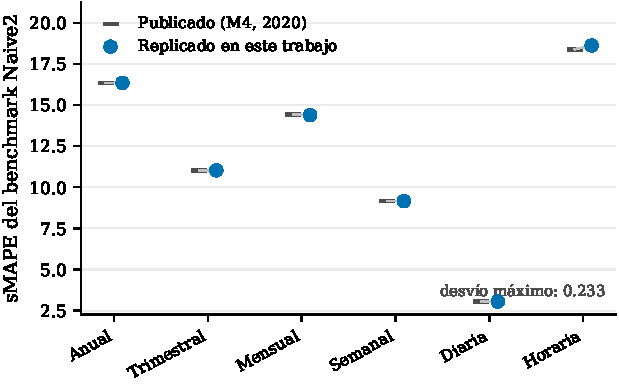
\includegraphics[width=0.62\linewidth]{figuras/fig9_validacion_naive2.pdf}
\caption{The replicated Naive2 benchmark against the one published by the competition.
The frequencies with $m=1$ match exactly.}
\label{fig:naive2}
\end{figure}

% =====================================================================

\section{Catastrophic failures versus mediocre ones}\label{sec:extremos}

Four models show OWA between 11 and 365, values that at first sight suggest an unusable
performance. Their medians, however, sit between $0.9$ and $1.8$: the mean is dominated
by a small number of series (Table~\ref{tab:extremos}).

\begin{table}[htbp]
\centering
\caption{Models whose mean MASE is dominated by extreme cases. The last column counts
the series with $\mathrm{MASE}>100$ out of a total of 5{,}773.}
\label{tab:extremos}
\begin{tabular}{lrrr}
\toprule
\textbf{Model} & \textbf{Mean MASE} & \textbf{Median MASE} & \textbf{Extreme series} \\
\midrule
ARIMA-NN     & 1{,}782.3 & 1.57 & 3 \\
LSTM         & 289.6     & 2.51 & 32 \\
LSTM-Conv1D  & 136.1     & 2.58 & 21 \\
SARIMA-NN    & 51.8      & 1.37 & 17 \\
Holt         & 7.5       & 1.71 & 118 \\
\bottomrule
\end{tabular}
\end{table}

The mechanism is an asymmetry between the two metrics: \textbf{sMAPE is bounded at 200,
MASE has no upper bound}. A forecast that diverges saturates in the sMAPE and drags the
mean MASE without limit. The witness case is series \texttt{H366}, where SARIMA produces
sMAPE $=199.99$ ---practically the largest possible value--- and MASE $=127{,}224$; that
single series accounts for the whole mean MASE of the hourly frequency.

Of Holt's 118 extreme cases, 117 are hourly: the model extrapolates a linear trend 48
steps ahead over series with a daily cycle, and diverges.

The most striking case by magnitude is SARIMA-NN in the monthly frequency, with
$\mathrm{OWA}=114.82$. The figure seems to rule the model out, but its median MASE in
that frequency is $0.83$ ---that is, \emph{better than the benchmark on the typical
series}--- and the mean of $236.7$ comes from 13 series out of 1{,}000. It is the same
tail mechanism described above taken to the extreme, and it is the reason why
Section~6.5 of the article places it fourth by ranks despite its being last by OWA.

The practical implication is direct. For production use, a model that fails
catastrophically on 0.3\% of the cases is \emph{less} preferable than one that is
consistently mediocre, because the failure cannot be detected beforehand. When reporting
a mean MASE it is worth accompanying it with the median and with the count of extreme
cases.

\paragraph{A third failure mode: structural inability.} The cases above share the
property that the model works well typically and goes out of control on a few series.
LightGBM, with an overall OWA $=1.702$, the worst in the bank, answers to a different
mechanism that is worth separating because it reads differently. Its failure is not in
the tail but in the center of the distribution, and it is not uniform across
frequencies: in monthly and quarterly its median sMAPE is $9.9$ and $9.2$, competitive;
in yearly and hourly it is $30.7$ and $20.4$, far behind the benchmark. The explanation
is a property of the model and not of its implementation: \textbf{an ensemble of trees
predicts leaf averages and by construction cannot extrapolate outside the observed
range}.

The evidence is direct. In the yearly frequency, whose median series has barely 29
observations, LightGBM issues a \emph{flat} forecast ---coefficient of variation below
$10^{-3}$ along the horizon--- on 95.7\% of the series, against 12.5\% for ARIMA. With
so few training rows left after building the lags, the trees find no splits with enough
support and collapse to a constant close to the sample mean. Naive2 is also constant in
that frequency, but it is constant \emph{at the last value}, which on series with a
trend is a far better constant. In the hourly frequency the forecast is not flat but
damped: its median coefficient of variation is $0.038$ against $0.201$ for the
benchmark, which is to say that it reproduces the daily cycle with a fifth of the
amplitude the series actually has.

This does not invalidate the evaluation: LightGBM was fitted with random search over
the same hyperparameter space as the other machine-learning methods (supplementary
material), and its result is the one that corresponds to applying an ensemble of trees
to short series with a trend and to long horizons with marked seasonality. Reporting it
is valuable precisely for that reason: \textbf{the distinction between a badly tuned
model and a model that is structurally inadequate for a family of series is exactly the
kind of heterogeneity that a decision rule conditioned on structure ought to capture},
and it explains why LightGBM never appears in the sets that Section~7.3 of the article
selects for yearly or hourly.


\begin{table}[htbp]
\centering
\caption{Sensitivity to the number of complexity strata. The advantage column is the
OWA difference between rule B and rule C; positive values favor the index.}
\label{tab:estratos}
\begin{tabular}{crrcr}
\toprule
\textbf{Strata} & \textbf{OWA of C} & \textbf{Advantage over B} &
\textbf{C better in} & \textbf{$p$} \\
\midrule
\textbf{2} & \textbf{0.8835} & \textbf{$+0.0306$} & \textbf{30/30} & $1.9\times10^{-9}$ \\
3 & 0.8898 & $+0.0243$ & 30/30 & $1.9\times10^{-9}$ \\
4 & 0.8853 & $+0.0287$ & 30/30 & $1.9\times10^{-9}$ \\
5 & 0.8918 & $+0.0223$ & 29/30 & $3.8\times10^{-6}$ \\
\bottomrule
\end{tabular}
\end{table}


\begin{table}[htbp]
\centering
\caption{Stability of the complexity index under perturbations, over 300 series per
frequency. Each cell is the percentage of series that crosses the median cut when the
index is recomputed on the perturbed series, and in parentheses the Spearman
correlation between the original index and the perturbed one. The cut is always set
with the original index.}
\label{tab:estabilidad}
% Siete columnas no caben a 11pt: a cuerpo normal se sale 37pt del margen.
\small
\setlength{\tabcolsep}{4.5pt}
\begin{tabular}{lrrrrrr}
\toprule
\textbf{Perturbation} & \textbf{Yearly} & \textbf{Quarterly} & \textbf{Monthly} & \textbf{Weekly} & \textbf{Daily} & \textbf{Hourly} \\
\midrule
Noise 1\% & 2.0 (0.990) & 1.3 (0.997) & 1.3 (0.998) & 1.7 (0.997) & 1.7 (0.994) & 0.3 (0.999) \\
Noise 2\% & 3.7 (0.987) & 1.0 (0.997) & 2.0 (0.997) & 2.7 (0.996) & 3.0 (0.993) & 1.0 (0.996) \\
Noise 5\% & 6.3 (0.979) & 2.7 (0.989) & 3.3 (0.993) & 5.8 (0.993) & 8.0 (0.984) & 2.7 (0.990) \\
\midrule
History 75\% & 16.3 (0.899) & 17.7 (0.865) & 26.0 (0.800) & 14.3 (0.841) & 28.3 (0.657) & 10.7 (0.960) \\
History 50\% & 33.1 (0.701) & 37.3 (0.642) & 37.7 (0.641) & 28.9 (0.577) & 41.3 (0.278) & 17.3 (0.939) \\
\bottomrule
\end{tabular}
\end{table}


% =====================================================================
\section{Why the classifier fails}\label{sec:clasificador}
% =====================================================================

Section~7.2 of the article reports that policy E ---a random forest that predicts
\emph{which} model wins on each series--- ends at OWA $1.4927$, worse than not routing at
all, and attributes the failure to the instability of the label. The explanation is
plausible and it is not the only one: there are at least four candidates, all four
predict the same failure, and they are told apart by what happens when each one is
corrected. This section puts them to the test over the same 30 partitions, the same
bank, the same forest of 300 trees and the same seed, so that row E of
Table~\ref{tab:clasificador} reproduces the published value digit by digit.

\paragraph{Class imbalance is not the cause.} The label spreads 27 models with a
normalized entropy of $0.911$ and a majority class of 13.5\%: the problem is not
degenerate. Retraining with balanced class weights lowers the \emph{mean} from $1.4927$
to $1.0453$, but raises the \emph{median} from $0.9851$ to $1.0233$. It does not fix the
typical partition ---it makes it worse---; all it does is cut the tail, because the
maximum across partitions goes from $15.21$ to $1.18$. Imbalance explains the variance
of the failure, not the failure.

\paragraph{The dominant cause is the asymmetry of the costs.} Classification minimizes
the $0$--$1$ loss: picking the wrong model always costs the same. But picking the second
best costs thousandths and picking one that diverges costs orders of magnitude
(Section~\ref{sec:extremos}). The damage turns out to be concentrated indeed: the worst
0.1\% of the series contributes 22.3\% of the excess OWA over the by-frequency policy,
the worst 1\% contributes 40.1\% and the worst 5\% contributes 67.8\%
(Figure~\ref{fig:clasificador}). Dropping from each policy its own worst 1\%, the
classifier goes from $1.4927$ to $0.8831$ and stops being catastrophic.

The decisive cut, however, is corrective and not descriptive. Keeping the same forest
and the same label ---with all its noise--- and changing \emph{only} the decision rule,
from keeping the most probable class to minimizing the expected regret
$\sum_c p(c\mid x)\,L[c,m]$, with $L[c,m]$ the mean regret of choosing $m$ among the
training series whose winner is $c$, the OWA goes from $1.4927$ to $\mathbf{0.8661}$:
better than the index ($0.8835$, in all 30 partitions, $p=1.9\times10^{-9}$) and better
than the per-model regressor ($0.8746$, in 22 of 30, $p=5.6\times10^{-4}$).

Two controls rule out the easy readings. If $p(c\mid x)$ is replaced by the training
proportion ---the same cost matrix, without looking at the features--- the OWA is
$0.9165$, which is the by-frequency rule: the cost structure on its own buys nothing,
and the features contribute $0.0504$ of the $0.0573$ that separate $E_3$ from the fixed
model. And if the matrix is estimated once for all frequencies instead of one per
frequency, the OWA is $0.8814$, still ahead of the index: the result does not depend on
conditioning by frequency.

\paragraph{The probabilities are calibrated, and policy E discards them.} The accuracy of
the classifier is 18.5\% ---40.7\% if the top-3 is allowed--- and its mean confidence is
$0.206$, with an expected calibration error of $0.023$. The forest, put another way,
\emph{knows that it does not know}, and policy E throws that information away by keeping
the most probable class. A rule with abstention ---use the winner of the frequency when
confidence does not reach $\tau$--- reaches $0.9016$ with $\tau=0.25$, abstaining on 77\%
of the series. It is better than not routing and far inferior to correcting the loss:
calibration is usable, but it is not where the problem lies.

\paragraph{The label is indeed almost arbitrary, and even so it is not what sinks the
OWA.} On 11.5\% of the series the first and the second have the \emph{same} sMAPE
---models that collapse to the same forecast--- and on 24.6\% less than 1\% separates
them, with a median of 5.9\%. The label is unstable to that extent, and that bounds the
achievable accuracy regardless of which classifier is used. What the preceding evidence
shows is that the low accuracy is not what produces the $1.49$: with the same label and
the same forest, changing the decision rule is enough to reach $0.8661$.

\paragraph{What this corrects in the reading of the article.} The design recommendation
survives ---predicting the error of each candidate and keeping the smallest is robust;
predicting the winner and believing it is not--- but its reason changes. The regression
formulation does not dominate because the label is noise, but because it \textbf{encodes
the loss}; classification with the loss encoded dominates both. It is also worth not
reading the 15.0\% of $E_3$ alongside the figures of Section~7.3 of the article: that
experiment draws the partitions differently and therefore has a different oracle bound,
so its figures are comparable within it and not across experiments.

\begin{table}[htbp]
\centering
\caption{The four explanations of the classifier's failure, put to the test. Every row
shares the 30 partitions, the bank, the forest of 300 trees and the seed; row E
reproduces the value of Table~5 of the article. The closing column is the fraction of
the gap between the fixed model ($0.9234$) and the per-series oracle ($0.5423$).}
\label{tab:clasificador}
\begin{tabular}{llrrrr}
\toprule
& \textbf{Variant} & \textbf{OWA} & \textbf{Median} & \textbf{s.d.} & \textbf{Closes} \\
\midrule
E & Classifier, most probable class & 1.4927 & 0.9851 & 2.592 & $-152.2$\% \\
\midrule
\multicolumn{6}{@{}l}{\emph{(1) Class imbalance}}\\
$E_1$ & Balanced class weights & 1.0453 & 1.0233 & 0.066 & $-32.0$\% \\
\multicolumn{6}{@{}l}{\emph{(2) Heterogeneous error costs}}\\
$E_2$ & Labels pruned to 10 models & 0.9152 & 0.9175 & 0.017 & $2.1$\% \\
$E_3$ & Bayes decision with costs & \textbf{0.8661} & 0.8659 & 0.006 & \textbf{15.0}\% \\
\multicolumn{6}{@{}l}{\emph{(3) Calibration}}\\
$E_4$ & Abstention below $\tau=0.25$ & 0.9016 & 0.8956 & 0.024 & $5.7$\% \\
\midrule
\multicolumn{6}{@{}l}{\emph{Controls on $E_3$}}\\
 & No features, proportion only & 0.9165 & 0.9151 & 0.007 & $1.8$\% \\
 & Single matrix, no frequency & 0.8814 & 0.8808 & 0.008 & $11.0$\% \\
\midrule
\multicolumn{6}{@{}l}{\emph{Reference rows from Table~5 of the article}}\\
B & By frequency & 0.9140 & 0.9140 & 0.007 & $2.4$\% \\
C & Frequency $\times$ index & 0.8835 & 0.8832 & 0.006 & $10.5$\% \\
F & Per-model regressor & 0.8746 & 0.8730 & 0.014 & $12.8$\% \\
\bottomrule
\end{tabular}
\end{table}

\begin{figure}[htbp]
\centering
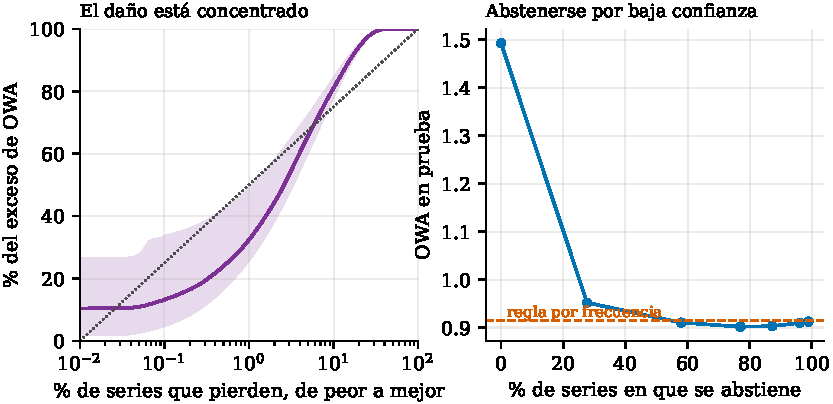
\includegraphics[width=\linewidth]{figuras/fig16_clasificador.pdf}
\caption{Left: fraction of the excess OWA over the by-frequency policy contributed by
the series ordered from worst to best, within each partition. The line is the median of
the 30 curves and the band the interquartile range; the dotted diagonal would be damage
spread evenly. The curve is computed partition by partition because pooling the 30 is
not informative: a single series from the partition that blows up to $15.21$ takes two
thirds of the accumulated excess. Right: OWA of the rule with abstention as a function
of the fraction of series on which it abstains.}
\label{fig:clasificador}
\end{figure}


\section{Validation outside M4}\label{sec:m3}
% =====================================================================

The whole article takes place inside M4: the index is built with M4, the cuts are set
with M4 and the policies are trained and tested on halves of M4. The objection is
immediate ---how much of all this is M4--- and it admits an answer that requires no
retraining at all. The M3 competition published the \emph{forecasts} of the methods that
competed, series by series and horizon by horizon (Makridakis and Hibon, 2000;
distributed in the \texttt{Mcomp} package, both cited in the article), so that the error
per series and per model can be reconstructed without fitting a single new model. That is
what is pertinent when the question is whether the \emph{rule} transfers and not whether
one knows how to train models. Two of the 24 methods ---AAM1 and AAM2--- forecast only
the quarterly and monthly series, and the protocol requires the complete bank on every
series: 22 methods remain over the 3,003 series, with NAIVE2 inside the bank and at the
same time as the denominator of the OWA, just as naive2 is in M4.

The descriptors are computed with the same code that computed them on M4, and the index
is \textbf{transferred}: the imputation medians, the means and scales of the
standardizer and the PC1 loadings are estimated on M4 and applied to M3 without
refitting. That is what makes this an external test and not a refit under another name.
Two checks support the setup: when the fit is redone on M4 the recomputed index matches
the stored one to a maximum difference of $5.3\times10^{-15}$, and the OWA reconstructed
on M3 places THETA first (0.8516), the method that performed best in that competition.
The OWA levels of M3 and M4 are not comparable with each other ---different bank,
different size, different frequencies and a different oracle--- and they are not
compared: what is comparable is the structure, that is, which claims repeat and what
fraction of the gap to the oracle is left untraveled.

\paragraph{The index transfers as a measure of difficulty.} PC1 explains 28.1\% of the
variance in M3 against 26.9\% in M4, and the transferred index correlates $0.995$ with
the one obtained by re-estimating everything inside M3: the covariance structure of the
29 descriptors is practically the same in the two collections. And it orders by
difficulty equally well or better: the Spearman correlation with the naive sMAPE is
$+0.488$ in M3 against $+0.410$ in M4, and the first decile of the index has an error of
one third of its collection's mean while the last almost doubles it, in both
(Figure~\ref{fig:m3}c).

\paragraph{And it does not transfer as a routing key.} Policy C ---stratifying by
frequency and by the median of the index--- travels 10.5\% of the gap to the oracle in
M4 and only 1.9\% in M3, with an advantage over the by-frequency rule in 22 of 30
partitions ($p=0.028$). With the index re-estimated inside M3 the advantage drops to 21
of 30 and stops being significant ($p=0.10$), so that what does not transfer is not the
index: it is that there be anything to gain by stratifying. This is the strongest
limitation the work finds against itself, and it is worth stating without softening it:
\textbf{the index measures difficulty in both collections and in only one of them does
that turn into a better choice of model}.

\paragraph{The margin is set by the bank, not by the series.} The reason lies not in the
series of M3 but in its methods. Five of the 22 come within 5\% of the best ---in M4
only two of 27 are that close to the best--- and THETA wins almost everywhere: barely 4
of the 8 cells of policy C choose something other than the global winner, against 9 of
12 in M4. It is not that the series of M3 are more homogeneous; in fact the oracle label
is more spread out there (normalized entropy $0.967$ and a majority class of 7.5\%,
against $0.911$ and 13.5\% in M4). What is more homogeneous is the bank. Routing can only
buy something if the candidates differ enough from one another, and that is a property of
the bank one chooses, not of the collection one forecasts.

\paragraph{The correction of Section~\ref{sec:clasificador} transfers, and with no models
that diverge.} Policy E again lands below the by-frequency rule, now in 28 of 30
partitions ($p=1.9\times10^{-8}$), and changing only the decision rule ---the same
forest, the same label, the expected regret instead of the most probable class--- takes
it from $0.8725$ to $0.8322$, ahead of the index in 27 of 30 ($p=1.7\times10^{-6}$). How
it happens matters: in M3 \emph{no} candidate blows up. The worst of the 22 methods ends
at OWA $1.022$, whereas in M4 six of the 27 models exceed OWA $2$ and the worst reaches
$271.8$. The natural objection to Section~\ref{sec:clasificador} ---that the problem of
the $0$--$1$ loss reduces to a few catastrophic candidates--- is thereby ruled out: the
asymmetry of the costs is enough to sink the classifier in a bank where nothing
diverges.

\paragraph{What does not hold outside M4.} That the cost-sensitive classifier beats the
per-model regressor is a result of M4. In M3 the two policies tie ($0.8322$ against
$0.8293$, 11 of 30 partitions in favor of the classifier, $p=0.29$). The claim that
survives the change of collection is the weaker of the two, and it is the one worth
making: once the loss is encoded, classifying and regressing arrive at the same place,
and choosing between them is a matter of convenience and not of principle.

\paragraph{The ceiling is worse outside.} In M3 the best of the policies leaves 93.3\% of
the gap between the fixed model and the per-series oracle unrecovered; in M4, 85.0\%. The
central result of the article not only survives the change of collection: it is more
severe outside than inside, and it is so against a bank of methods that was not chosen
here and over which no decision of this work could have any influence.

\begin{table}[htbp]
\centering
\caption{The policies of Table~5 of the article, repeated over the 3,003 series of M3
with the published forecasts of 22 methods and the same protocol of 30 partitions. The
OWA values of the two blocks are \textbf{not} comparable with each other ---different
bank and different oracle---; what is comparable is the closing column, the fraction of
the gap between the fixed model and the oracle that each policy travels. The index used
in M3 is the one from M4, transferred without refitting.}
\label{tab:m3}
\begin{tabular}{llrrrr}
\toprule
& & \multicolumn{2}{c}{\textbf{M4} · 27 models}
  & \multicolumn{2}{c}{\textbf{M3} · 22 methods} \\
\cmidrule(lr){3-4}\cmidrule(lr){5-6}
& \textbf{Policy} & \textbf{OWA} & \textbf{Closes} & \textbf{OWA} & \textbf{Closes} \\
\midrule
A & Fixed model & 0.9234 & --- & 0.8527 & --- \\
B & By frequency & 0.9140 & 2.4\% & 0.8492 & 1.0\% \\
C & Frequency $\times$ index & 0.8835 & 10.5\% & 0.8460 & 1.9\% \\
E & Classifier & 1.4927 & $-152.2$\% & 0.8725 & $-5.8$\% \\
E$'$ & Cost-sensitive classifier & \textbf{0.8661} & \textbf{15.0}\% & 0.8322 & 5.9\% \\
F & Per-model regressor & 0.8746 & 12.8\% & \textbf{0.8293} & \textbf{6.7}\% \\
D & Oracle (bound) & 0.5423 & 100\% & 0.5078 & 100\% \\
\bottomrule
\end{tabular}
\end{table}

\begin{figure}[htbp]
\centering
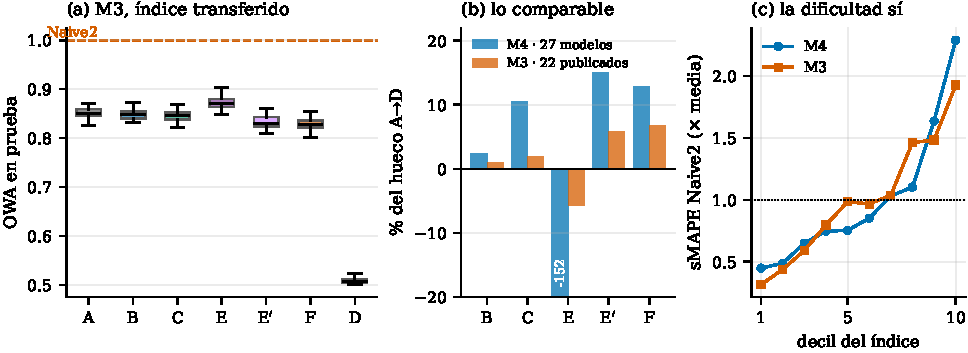
\includegraphics[width=\linewidth]{figuras/fig17_validacion_m3.pdf}
\caption{(a) The policies over M3, with the index transferred from M4. (b) The only
legitimate comparison between the two collections: not the OWA but the fraction of the
gap between the fixed model and the oracle that each policy travels; the bar for E in M4
is $-152$\% and is clipped. (c) What does transfer: the naive sMAPE by decile of the
index, in multiples of each collection's mean.}
\label{fig:m3}
\end{figure}


\appendix
\section{Model configuration}\label{ap:hiperparametros}
% =====================================================================

Table~\ref{tab:hiperparametros} details the configuration of the 27 models. The values
are not transcribed from the libraries' documentation but from the configuration
recorded in each run, so that they reflect what was actually executed. For the models
fitted by random search the search space is reported and not the selected value, which
differs across series. The architectures of the neural networks were obtained by
instantiating each model and reading off its layers.

% Tabla de hiperparametros, version en ingles de apendice_hiperparametros.tex
% Requiere: \usepackage{booktabs}, \usepackage{longtable} y \usepackage{array}
% Las columnas van en ragged right: justificado en una columna angosta
% deja huecos y LaTeX lo reporta como underfull hbox.
%
% OJO: el porcentaje de validacion va como 20\%, no 20\\% -- el doble
% backslash cerraba la fila y el % comentaba el resto, que es como se
% perdieron los conteos de parametros entrenables en el original.
\begin{longtable}{>{\raggedright\arraybackslash}p{0.21\linewidth}>{\raggedright\arraybackslash}p{0.71\linewidth}}
\caption{Configuration of the 27 models evaluated. The values come from the configuration actually recorded in each run, not from the libraries' documentation. ``per series'' indicates that the parameter is selected automatically for each series.}\label{tab:hiperparametros}\\
\toprule
\textbf{Model} & \textbf{Configuration} \\
\midrule
\endfirsthead
\toprule
\textbf{Model} & \textbf{Configuration} \\
\midrule
\endhead
\bottomrule
\endfoot
\multicolumn{2}{l}{\textit{Benchmark}} \\[1mm]
\hspace{.6em}Naive & Repeats the last observation \\
\hspace{.6em}Seasonal naive & period = 4 \\
\addlinespace
\multicolumn{2}{l}{\textit{Statistical}} \\[1mm]
\hspace{.6em}Exponential smoothing & alpha\_optimized: per series \\
\hspace{.6em}Holt & alpha\_optimized: per series; beta\_optimized: per series \\
\hspace{.6em}Holt-Winters & alpha: per series; beta: per series; gamma: per series \\
\hspace{.6em}ARIMA & p\_d\_q: per series; P\_D\_Q\_m: per series \\
\hspace{.6em}SARIMA & p\_d\_q: per series; P\_D\_Q\_m: per series \\
\hspace{.6em}ETS & alpha: per series; use\_boxcox = False \\
\addlinespace
\multicolumn{2}{l}{\textit{Machine learning}} \\[1mm]
\hspace{.6em}Linear regression & fit\_intercept = True; tol = 1e-06 \\
\hspace{.6em}LassoLars & Fitted per series with RandomizedSearchCV (25 draws, 3-fold cross-validation) over: alpha $\in$ logspace($-4$, 1, 60); max\_iter $\in$ \{200, 500, 1000, 2000\}; fit\_intercept, positive, precompute \\
\hspace{.6em}Bayesian ridge & Fitted per series with RandomizedSearchCV (25 draws, 3-fold cross-validation) over: alpha$_1$, alpha$_2$, lambda$_1$, lambda$_2$ $\in$ logspace($-8$, $-2$, 20); tol $\in$ \{1e-6, 1e-5, 1e-4, 1e-3\} \\
\hspace{.6em}Bagging & Fitted per series with RandomizedSearchCV (30 draws, 3-fold cross-validation) over: n\_estimators $\in$ \{50, 100, 200, 300, 500\}; max\_samples and max\_features $\in$ \{0.5, 0.7, 0.9, 1.0\}; bootstrap \\
\hspace{.6em}Random Forest & Fitted per series with RandomizedSearchCV (30 draws, 3-fold cross-validation) over: n\_estimators $\in$ \{50, 100, 200, 300\}; max\_depth $\in$ \{None, 5, 10, 20, 30\}; min\_samples\_split, min\_samples\_leaf; max\_features $\in$ \{sqrt, log2, None\} \\
\hspace{.6em}AdaBoost & Fitted per series with RandomizedSearchCV (30 draws, 3-fold cross-validation) over: n\_estimators $\in$ \{50, 100, 200, 300, 500\}; learning\_rate $\in$ \{0.01, 0.05, 0.1, 0.2, 0.5, 1.0\}; loss $\in$ \{linear, square, exponential\}; depth of the base tree $\in$ \{2--6, None\} \\
\hspace{.6em}XGBoost & Fitted per series with RandomizedSearchCV (30 draws, 3-fold cross-validation) over: n\_estimators $\in$ \{100, 200, 300, 500\}; learning\_rate $\in$ \{0.01, 0.05, 0.1, 0.2\}; max\_depth $\in$ \{3, 5, 7, 10\}; subsample and colsample\_bytree $\in$ \{0.6, 0.8, 1.0\} \\
\hspace{.6em}LightGBM & Fitted per series with RandomizedSearchCV (30 draws, 3-fold cross-validation) over: n\_estimators $\in$ \{300, 600, 900\}; learning\_rate $\in$ \{0.02, 0.05, 0.1\}; max\_depth $\in$ \{4, 6, 8\}; num\_leaves $\in$ \{15, 31, 63\}; min\_data\_in\_leaf, max\_bin \\
\hspace{.6em}SVM & Fitted per series with RandomizedSearchCV (30 draws, 3-fold cross-validation) over: RBF kernel; $C \in$ \{0.1, 1, 10\}; epsilon $\in$ \{0.01, 0.1\}; gamma $\in$ \{scale, 0.01, 0.1\} \\
\hspace{.6em}KNN & Fitted per series with RandomizedSearchCV (30 draws, 3-fold cross-validation) over: n\_neighbors $\in$ \{1, \dots, 30\}; weights $\in$ \{uniform, distance\}; $p \in$ \{1, 2\} \\
\hspace{.6em}Gaussian process & Fitted per series with RandomizedSearchCV (30 draws, 3-fold cross-validation) over: kernel among combinations of RBF, Mat\'ern and WhiteKernel; alpha $\in$ \{1e-8, 1e-6, 1e-4, 1e-3\} \\
\addlinespace
\multicolumn{2}{l}{\textit{Hybrid}} \\[1mm]
\hspace{.6em}ARIMA-RF & arima\_order = (2, 1, 2); max\_lag = 3 \\
\hspace{.6em}ARIMA-NN & arima\_order = (2, 1, 2); max\_lag = 3 \\
\hspace{.6em}SARIMA-NN & sarima\_order = (2, 1, 2); seasonal\_order = (1, 1, 1, 4) \\
\addlinespace
\multicolumn{2}{l}{\textit{Neural network}} \\[1mm]
\hspace{.6em}Perceptron & Dense(64) $\to$ Dense(32) $\to$ Dense(1). Adam optimizer, MSE loss, 50 epochs, batch 16, validation 20\%. 2,561 trainable parameters \\
\hspace{.6em}1D ConvNet & Conv1D(64) $\to$ Dropout(0.1) $\to$ Flatten $\to$ Dense(32) $\to$ Dense(1). Adam optimizer, MSE loss, 50 epochs, batch 16, validation 20\%. 13,569 trainable parameters \\
\hspace{.6em}LSTM & Bidirectional $\to$ Dropout(0.1) $\to$ LSTM(64) $\to$ Dense(32) $\to$ Dense(32) $\to$ Dense(1). Adam optimizer, MSE loss, 50 epochs, batch 16, validation 20\%. 88,929 trainable parameters \\
\hspace{.6em}Transformer & Dense(64) $\to$ LayerNormalization $\to$ MultiHeadAttention $\to$ Dropout(0.1) $\to$ Add $\to$ LayerNormalization $\to$ Dense(128) $\to$ Dropout(0.1) $\to$ Dense(64) $\to$ Add $\to$ LayerNormalization $\to$ MultiHeadAttention $\to$ Dropout(0.1) $\to$ Add $\to$ LayerNormalization $\to$ Dense(128) $\to$ Dropout(0.1) $\to$ Dense(64) $\to$ Add $\to$ Lambda $\to$ Dense(128) $\to$ Dropout(0.1) $\to$ Dense(1). Adam optimizer, MSE loss, 50 epochs, batch 16, validation 20\%. 75,841 trainable parameters \\
\hspace{.6em}LSTM-ConvNet & Conv1D(64) $\to$ Bidirectional $\to$ Dropout(0.1) $\to$ LSTM(50) $\to$ Dense(64) $\to$ Dense(32) $\to$ Dense(1). Adam optimizer, MSE loss, 50 epochs, batch 16, validation 20\%. 82,793 trainable parameters \\
\addlinespace
\end{longtable}



% =====================================================================
\section{Environment and reproducibility details}\label{ap:repro}
% =====================================================================

The results of Section~7.6 of the article are claims about reproducibility, so the
environment in which they were obtained is part of the result and not of the
administrative annex.

\paragraph{Environment.} Python 3.10.20 on macOS ARM64 (Apple Silicon), TensorFlow
2.21.0, NumPy 2.2.5, scikit-learn 1.7.2 and statsmodels 0.14.6. All the computation was
carried out on CPU; no GPU was involved at any stage, so the sources of nondeterminism
associated with GPU kernels do not apply to what is reported.

\paragraph{Architectures and training.} Table~\ref{tab:hiperparametros} details the
layers, optimizer, loss function, number of epochs, batch size, validation split and
number of trainable parameters of each network. All five are trained with Adam and MSE
loss for 50 epochs, batch 16 and 20\% validation, without early stopping. The winning
model of each series in the seed experiment is determined by the sMAPE over the official
M4 test set, not by the validation loss: the question is which architecture \emph{would
have been reported as best}, and that decision is usually taken on the evaluation
metric.

\paragraph{Seed experiment.} 30 series from each of the six frequencies (180 in all)
$\times$ 5 seeds $\times$ 5 architectures $=4{,}500$ measurements. Across runs the data
split, the features, the scaling and all the hyperparameters are held fixed; the only
thing that varies is the argument of \texttt{tf.random.set\_seed} and
\texttt{numpy.random.seed}.

\paragraph{The thread-count experiment.} The re-run that reproduced none of the
2{,}250 measurements differs from the original in a single respect: the environment
variables \texttt{OMP\_NUM\_THREADS}, \texttt{MKL\_NUM\_THREADS} and
\texttt{OPENBLAS\_NUM\_THREADS} went from 4 to 2, with identical seeds, versions and
data. \texttt{tf.config.experimental.enable\_op\_determinism()} was \textbf{not} active
in either condition, which is precisely the default setting under which most published
work is run and the reason why the result is pertinent: fixing the seed, as was done,
turned out to be insufficient. The largest difference observed between runs was 105.8
sMAPE points on one series, while the aggregate statistic ---the share of series where
the winning architecture changes--- moved from 68\% to 67\%.

\paragraph{What reproduces exactly and what does not.} The deterministic stages of the
processing ---extraction of the 29 descriptors, standardization, PCA, index, cluster
assignment, the three entropies and the forecast errors of the statistical and
machine-learning models--- reproduce with a difference of $0.00$ over the 99{,}935
series when re-run. The stages that involve neural networks do not reproduce, and that
asymmetry is the content of Section~7.6 of the article.

\begin{table}[htbp]
\centering
\caption{Correlation of the index with two different targets, over the 4,708 series
evaluated with the 27 models.}
\label{tab:oraculo}
\begin{tabular}{lcc}
\toprule
\textbf{Target} & \textbf{Pearson} & \textbf{Spearman} \\
\midrule
Error of the naive forecast        & 0.435 & 0.449 \\
\textbf{Error of the best available model} & \textbf{0.439} & \textbf{0.502} \\
\bottomrule
\end{tabular}
\end{table}

\begin{figure}[htbp]
\centering
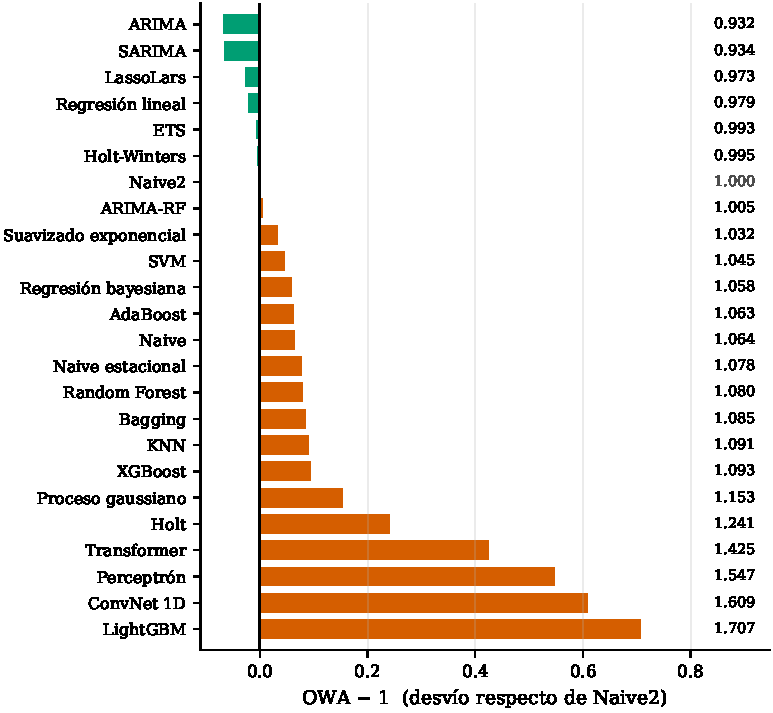
\includegraphics[width=0.72\linewidth]{figuras/fig6_owa_modelos.pdf}
\caption{Deviation of the OWA from the Naive2 benchmark. In green the models that beat
it; in gray the benchmark itself. Four models with OWA $>3$ are omitted, whose means are
dominated by divergent fits (see Table~\ref{tab:extremos}).}
\label{fig:owa}
\end{figure}
